\subsection{Loop principal}
  Para esta parte, reutilizaremos el código del \cref{sec:Complicando_las_cosas}.

  \begin{kotlin}
    fun main() {
      println("Welcome to the Fibonacci Calculator!")
      println("Please enter a number to calculate the Fibonacci sequence for or 'q' to quit")
      while (true) {
        val input = readln()
        if (input == "q") {
          println("Goodbye!")
          break
        }
        val n = input.toInt()
        println("The Fibonacci number for $n is ${recursiveFibonacci(n)}")
      }
    }
  \end{kotlin}

  Veamos qué hace este código:
  \begin{itemize}
    \item Imprime un mensaje de bienvenida.
    \item Imprime un mensaje pidiendo un número.
    \item Inicia un loop infinito.
    \item Lee la entrada del usuario con la función \texttt{readln(): String}.
    \item Si la entrada es \texttt{q}, imprime un mensaje de despedida y sale del loop con la 
      palabra reservada \texttt{break}.
    \item Si la entrada no es \texttt{q}, convierte la entrada a un número y calcula el número de 
      Fibonacci para ese número.
    \item Imprime el resultado.
  \end{itemize}

  ¿Y si ahora queremos que el usuario pueda elegir entre calcular el número de Fibonacci de forma
  recursiva o iterativa?
  Para esto podemos utilizar una expresión \textit{if-else}, pero una forma más elegante de hacerlo
  es utilizando la expresión \textit{when}.

  \begin{kotlin}
    fun main() {
      println("Welcome to the Fibonacci Calculator!")
      println("""
        |Usage:
        |  - Enter a number to calculate the Fibonacci number
        |  - Enter 'r' to use the recursive algorithm
        |  - Enter 'i' to use the iterative algorithm
        |  - Enter 'q' to quit
        """.trimMargin())
      while (true) {
        when(readln()) {
          "q" -> {
            println("Goodbye!")
            break
          }
          "r" -> {
            println("Using recursive algorithm")
            println("Fibonacci number: ${recursiveFibonacci(readln().toInt())}")
          }
          "i" -> {
            println("Using iterative algorithm")
            println("Fibonacci number: ${iterativeFibonacci(readln().toInt())}")
          }
          else -> {
            println("Invalid input")
          }
        }
      }
    }
  \end{kotlin}

  Veamos las partes escenciales de este código:

  \begin{itemize}
    \item Primero notemos que el segundo print está escrito con triple comilla doble, esto se llama
      \textit{raw string literal} y nos permite escribir strings con saltos de línea y tabulaciones
      sin tener que escaparlos.
      La función \texttt{trimMargin()} elimina los espacios en blanco al inicio de cada línea.
      Para entender mejor lo que hace la función \texttt{trimMargin()}, podemos revisar la 
      documentación desde el IDE, para esto simplemente colocamos el cursor sobre la función como
      en la \cref{fig:trimMargin}.
    \item La expresión \textit{when} es una expresión que funciona como un \textit{if-else} pero con
      múltiples condiciones.
      En este caso, si la entrada es \texttt{q}, se imprime un mensaje de despedida y se sale del
      loop.
      Si la entrada es \texttt{r}, se imprime un mensaje indicando que se está usando el algoritmo
      recursivo, se lee un número y se calcula el número de Fibonacci para ese número.
      Si la entrada es \texttt{i}, se imprime un mensaje indicando que se está usando el algoritmo
      iterativo, se lee un número y se calcula el número de Fibonacci para ese número.
      Si la entrada no es ninguna de las anteriores, se imprime un mensaje indicando que la entrada
      es inválida.
  \end{itemize}

  \begin{figure}[ht!]
    \centering
    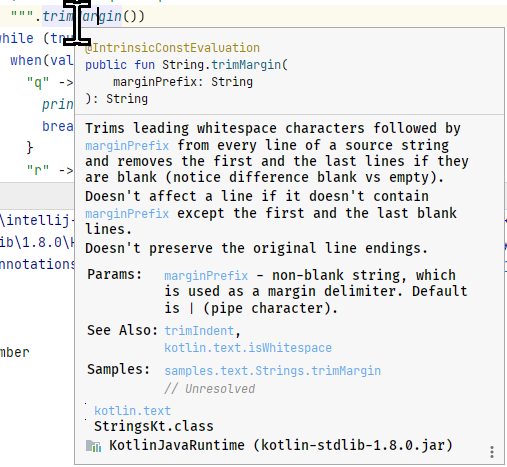
\includegraphics[width=0.5\textwidth]{img/Por_algo_se_empieza/trimMargin.png}
    \caption{Documentación de la función \texttt{trimMargin()}.}
    \label{fig:trimMargin}
  \end{figure}

  Con esto termina la parte introductoria de este libro, en la siguiente parte veremos cómo
  utilizar las herramientas de desarrollo que nos ofrece IntelliJ IDEA para crear aplicaciones
  más complejas y robustas, tratando de sacarle el máximo provecho a Kotlin e IntelliJ IDEA.

  Pero antes, algunos ejercicios para practicar lo que hemos visto hasta ahora \texttt{:)}